% chapters/ch4-sec2b.tex -- 2.3 Solutions for a Non-Oscillating Rocket in the Coasting Phase; 2.4 Numerical
% Methods for the Digital Computation of Altitude Performance; 2.5 Validity of the Approximate Methods Compared
% to Numerical Solutions by the Interval Method (PDF 571-596, printed pp. 539-564), up to but not including the
% heading "3." on PDF 596. Equations 61-89, Figures 3-4 and the panel Figures 5(a)-9(c), and the unnumbered key
% to Figures 5-9 (PDF 587).
\subsection{Solutions for a Non-Oscillating Rocket in the Coasting Phase}\label{ch4:sec:2.3}

The analyses of Sections~\ref{ch4:sec:2.1} and~\ref{ch4:sec:2.2} have been directed toward the
determination of the burnout altitude and burnout velocity of a vertically-launched model rocket that does
not experience any changes in angle of attack due to rigid-body rotations. The burning phase, however, tells
only half the story of a rocket's flight. After expending its propellant charge the model continues to coast
upward for a considerable distance until the momentum associated with its burnout velocity is reduced to
zero by the action of gravity and aerodynamic drag, at which time the \emph{apex}, or highest point in the
flight, occurs. In fact, as those who have seen model rockets in flight doubtless know, the coasted altitude
increment is usually considerably greater than the burnout altitude. In this section the differential
equation of point-mass motion will be solved to yield the two quantities of primary importance to a
knowledge of the coasting phase of a rocket's flight: the coasted altitude increment and the time interval
between the burnout of the uppermost stage and the flight apex.

After the burnout of the last stage, the vertical differential equation of motion becomes
\begin{equation}\label{ch4:eq:61}
m(t)\frac{dv}{dt} = -m(t)g - kv^{2}
\end{equation}
As we did for the burning-phase analyses, we shall make the approximation that the mass of the rocket
remains constant throughout the coasting phase of flight. The only change in mass that does in fact occur
after burnout is the slight mass loss due to the burning of the \emph{delay train}, or time delay charge, in
the engine. For all practical purposes this mass loss is negligible, so that $m(t)$ can be approximated by
the burnout mass $m_b$ and equation~\eqref{ch4:eq:61} becomes
\begin{equation}\label{ch4:eq:62}
m_b\frac{dv}{dt} = -m_b g - kv^{2}
\end{equation}
This relation may be rearranged to solve for $t$ as a function of $v$. Using the fact that the model's
velocity is reduced to zero at flight apex, one can then obtain the coasting time between burnout and apex
by solving
\begin{equation}\label{ch4:eq:63}
\int_{v_b}^{0}\frac{m_b\,dv}{-m_b g - kv^{2}} = \int_{0}^{t_c} dt
\end{equation}
which yields
\begin{equation}\label{ch4:eq:64}
t_c = \sqrt{\frac{m_b}{gk}}\,\tan^{-1}\left[v_b\sqrt{\frac{k}{m_b g}}\,\right]
\end{equation}

Equation~\eqref{ch4:eq:62} can also be solved for the coasted altitude increment by introducing the
following transformation of variables:
\begin{equation}\label{ch4:eq:65}
\frac{dv}{dt} = \frac{dv}{dy}\,\frac{dy}{dt} = v\frac{dv}{dy}
\end{equation}
When~\eqref{ch4:eq:65} is substituted into~\eqref{ch4:eq:62} and the resulting equation is solved for $y$
as a function of $v$ we obtain
\begin{equation}\label{ch4:eq:66}
\int_{v_b}^{0}\frac{v\,dv}{m_b g + kv^{2}} = \int_{0}^{y_c} -\frac{dy}{m_b}
\end{equation}
When integrated, \eqref{ch4:eq:66} yields the coasted altitude increment $y_c$ as
\begin{equation}\label{ch4:eq:67}
y_c = \frac{m_b}{2k}\ln\left[\frac{kv_b^{2}}{m_b g} + 1\right]
\end{equation}

The total altitude at apex is then just the sum of $y_c$ and the burnout altitude increments of all the
stages, while the total time elapsed from liftoff to apex is the sum of $t_c$ and the burning times of all
the stages. When using equation~\eqref{ch4:eq:64} to calculate the coasting time and
equation~\eqref{ch4:eq:67} to calculate the coasted altitude increment of the uppermost stage of a
multistaged rocket, it is important to note that the burnout mass, burnout velocity, and drag parameter
\emph{of that stage} must be used for $m_b$, $v_b$, and $k$, respectively. Figure~\ref{ch4:fig:3}
illustrates by example the synthesis of burning-phase and coasting-phase solutions to obtain the overall
performance and flight-time characteristics of a three-staged model rocket.

\begin{figure}[htbp]
  \centering
  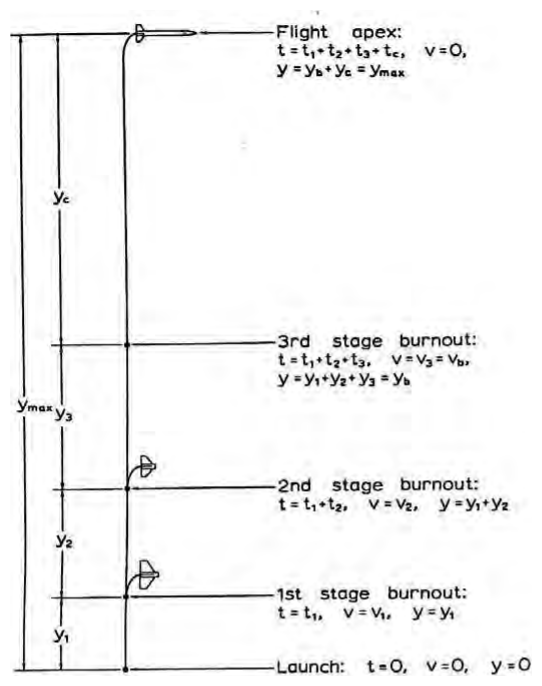
\includegraphics[width=0.8\textwidth,height=0.85\textheight,keepaspectratio]{figures/ch4/fig03.png}
  \caption{Assembly of burning-phase and coasting-phase solutions to obtain the total altitude and time to
    flight apex of a three-staged model rocket.}
  \label{ch4:fig:3}
\end{figure}

\subsection{Numerical Methods for the Digital Computation of Altitude Performance}\label{ch4:sec:2.4}

The preceding sections have described methods which can be used by the model rocketeer to give accurate
predictions of his vehicle's altitude capability with relatively little actual calculation. By this I
certainly do not mean to imply that the reader should find the solutions trivial to work; indeed, until you
have had some practice with them it is to be expected that you may find them somewhat difficult to handle.
But a human being who applies himself with a reasonable amount of diligence \emph{can} work them out in
fairly short order---and this fact alone indicates that there is little actual calculation involved,
considering the difficulty of the problem. The methods developed in Sections~\ref{ch4:sec:2.1}
through~\ref{ch4:sec:2.3} are, moreover, excellent approximations to the exact solution of the differential
equation of vertical motion, equation~\eqref{ch4:eq:12}, with $\alpha$ and $\theta$ both equal to zero. If
a more precise determination of the flight performance than that possible using the preceding methods
\emph{is} desired, \eqref{ch4:eq:12} can be solved to \emph{any} desired accuracy---but, since such a
solution requires the use of numerical methods involving a far greater amount of calculation than the
closed-form approximations, it becomes necessary to program the problem for solution on an automatic,
digital computer. This section will present two such methods, as well as some supplementary material on
engine thrust and mass functions.

Before we can obtain an accurate solution to the differential equation of motion, we require an accurate
knowledge of the thrust-vs.-time and mass-vs.-time curves for the rocket in question. This usually means
closed-form, analytic expressions for these curves, for although such curves can be represented by tables
which are read by the machine at any desired value of time most modelers who have used computers find the
tabular representation awkward and inconvenient in practice. For a rocket engine, as was shown in
Chapter~\ref{ch1}, we have the following relationship between thrust and mass loss:
\begin{equation}\label{ch4:eq:68}
F(t) = c\,\frac{dm_e}{dt}
\end{equation}
where $c$ is the exhaust velocity of the combustion products and $dm_e/dt$ is the mass flow rate at which
the combustion products are being expelled from the nozzle. For the great majority of model rocket engines,
the exhaust velocity does not vary greatly during the burn time and can be approximated by its average
value, which in turn can be calculated from the motor's specific impulse according to
\begin{equation}\label{ch4:eq:69}
c = g\Isp
\end{equation}
so that it is a simple matter to obtain $dm_e/dt$ from~\eqref{ch4:eq:68} once the analytic function
representing the variation of thrust with time is known. This, in turn, is fairly easily determined since
all manufacturers of model rocket engines give rather accurate data on the total impulse, maximum thrust,
average thrust, burn time, and general shape of the thrust-time curve of each type they produce. The rate
at which the mass of the rocket changes during the burning phase of flight is just equal to $-dm_e/dt$,
since the loss of combustion products through the nozzle is the only source of mass variation in virtually
all model rockets.

It will be recalled that typical thrust-time curves for model rocket engines were discussed in detail in
Chapter~\ref{ch1}, and that these curves fall into three basic categories:
\begin{enumerate}[label=(\alph*)]
  \item The curves of end-burning engines (most engines in NAR classes $\tfrac{1}{2}$A through C), which
    are characterized by relatively long burning times and relatively low, constant thrust except for a
    ``starting peak'' at ignition;
  \item The curve of the NAR type B14 engine, characterized by a rapid rise in thrust, an equally rapid
    decay in thrust, and a short burning time; and
  \item The curves of many engines in NAR classes D through F, whose conical-port grain geometries result in
    a thrust peak just before burnout, a relatively high average thrust, and a burn time intermediate
    between categories (a) and (b) above.
\end{enumerate}

The overwhelming majority of model rocket engines in common use are of the end-burning type where the
approximation of constant thrust is usually acceptable, and the mass expulsion rate may be regarded as
nearly constant throughout the burning time. The mass of a rocket using such an engine, as a function of
time, can then be written as
\begin{equation}\label{ch4:eq:70}
m(t) = m_o - \gamma t
\end{equation}
where $m_o$ is the rocket's mass at the instant of ignition and
\begin{equation}\label{ch4:eq:71}
\gamma = \frac{m_f}{t_b}
\end{equation}
where $m_f$ is the mass of the propellant charge and $t_b$ is the burning time.

The thrust-time and mass-time curves of \emph{any} engine type, end-burning or not, may be represented by
approximating the thrust-time curve by a closed-form, analytic function which satisfies the following basic
criteria:
\begin{enumerate}[label=(\alph*)]
  \item The total impulse of the mathematical representation chosen must equal the actual total impulse of
    the engine; i.e., if $F(t)$ is the mathematical representation,
    \begin{equation}\label{ch4:eq:72}
    I_t = \int_{0}^{t_b} F(t)\,dt
    \end{equation}
  \item The burning time of the mathematical representation must equal the actual burning time of the
    engine;
  \item The maximum thrust of the mathematical representation must equal the actual peak thrust of the
    engine; and
  \item The mathematical representation must equal the actual thrust of the engine at several points on the
    thrust-time curve or must be of the same general shape as the actual thrust-time curve, depending on the
    degree of accuracy desired.
\end{enumerate}

To approximate the actual thrust function, one may use a Fourier sine or cosine series, a polynomial fit,
or a combination of the two. Model rocket engines of any given type do exhibit a certain amount of variation
from one production article to the next, however, and it is not generally worthwhile to insist on too high
a degree of precision when constructing mathematical models of thrust-time curves---at least from the
standpoint of practical design. In fact, it turns out that the thrust-time curve of almost any model rocket
engine can be adequately approximated by a \emph{piecewise-linear} representation of the form
\begin{subequations}\label{ch4:eq:73}
\begin{align}
F(t) &= F_m\frac{t}{t_m} && (0 \le t \le t_m) \label{ch4:eq:73a}\\
F(t) &= F_m - \frac{t - t_m}{t_s - t_m}(F_m - F_s) && (t_m \le t \le t_s) \label{ch4:eq:73b}\\
F(t) &= F_s && (t_s \le t \le t_b) \label{ch4:eq:73c}
\end{align}
\end{subequations}
where
\begin{itemize}[nosep,leftmargin=*,label={}]
  \item $F_m$ = maximum thrust
  \item $F_s$ = sustainer thrust
  \item $t_m$ = time of occurrence of maximum thrust, and
  \item $t_s$ = time of onset of sustainer thrust
\end{itemize}
The corresponding functions for representing the model's mass as a function of time are
\begin{subequations}\label{ch4:eq:74}
\begin{align}
m(t) &= m_o - F_m\frac{t^{2}}{2ct_m} && (0 \le t \le t_m) \label{ch4:eq:74a}\\
m(t) &= m_o - \frac{F_m}{c}\left(t - \frac{t_m}{2}\right) + (F_m - F_s)\frac{(t - t_m)^{2}}{2c(t_s - t_m)}
  && (t_m \le t \le t_s) \label{ch4:eq:74b}\\
m(t) &= m_o - \frac{F_m t_s}{2c} - \frac{F_s(t_s - t_m)}{2c} - \frac{F_s}{c}(t - t_s)
  && (t_s \le t \le t_b) \label{ch4:eq:74c}
\end{align}
\end{subequations}
and the total impulse of the engine is given by
\begin{equation}\label{ch4:eq:75}
I_t = F_m\frac{t_s}{2} + F_s\left(t_b - \frac{t_m}{2} - \frac{t_s}{2}\right)
\end{equation}
The reader will recognize the notation used in equations~\eqref{ch4:eq:73} through~\eqref{ch4:eq:75} as
referring specifically to the end-burning engine with its characteristic initial thrust spike and clearly
identifiable sustainer thrust level; I repeat, however, that virtually any existing engine's
characteristics can be fairly well represented by this scheme. To approximate the thrust-time curve of a
core-burning motor like the B14, for instance, one would set $t_s$ equal to $t_b$ and $F_s$ equal to zero.
With $t_s$ and $F_s$ thus fixed it is no longer possible to satisfy our condition (c) above, but the error
in $F_m$ is insufficient to significantly affect performance calculations. In the case of the B14, for
instance, $F_m$ turns out to be 28.6 newtons, just over 10\% less than the nominal test value of 32
newtons---a representation that is certainly accurate enough for any calculations likely to be of interest
to the practical rocketeer. Figure~\ref{ch4:fig:4} illustrates by example the application of the
piecewise-linear method in approximating the thrust-time curve of a typical model rocket engine.

\begin{figure}[htbp]
  \centering
  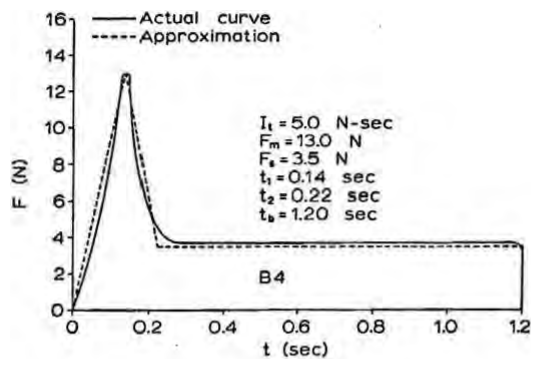
\includegraphics[width=0.8\textwidth,height=0.85\textheight,keepaspectratio]{figures/ch4/fig04.png}
  \caption{Approximating the thrust-time curve of a typical model rocket engine by a piecewise-linear fit.
    The parameters used in constructing an approximation to the thrust-time curve of the NAR Type B4 engine
    are shown along with the actual and approximate thrust-time curves.}
  \label{ch4:fig:4}
\end{figure}

We now proceed to the discussion of actual \emph{iteration} schemes for solving the differential equation
of vertical motion. At this stage in the development we can assume that all the functions and parameters of
the model and its rocket engine are known. The first iteration procedure consists of determining the
\emph{theoretical velocity increment} without drag over a small interval of time, adding this theoretical
increment to the velocity in the last interval, and determining the drag from the sum thus obtained. The
drag is then substituted back into the original force equation and the \emph{actual} velocity increment is
computed from the equation thus generated. The method works well for 0.1-second intervals, but intervals of
0.01 second are easily used on a digital computer and will yield greater accuracy. This method of
computation is outlined below:
\begin{align}
&\Delta v_t = \Delta t[F(t) - m(t)g]/m(t) \label{ch4:eq:76}\\
&\text{Drag} = k(v + \Delta v_t)^{2} \label{ch4:eq:77}\\
&\Delta v_a = \Delta t[F(t) - m(t)g - k(v + \Delta v_t)^{2}]/m(t) \label{ch4:eq:78}\\
&\Delta y = \Delta t[v + \Delta v_a/2] \label{ch4:eq:79}\\
&v = v + \Delta v_a \label{ch4:eq:80}\\
&y = y + \Delta y \label{ch4:eq:81}\\
&t = t + \Delta t \label{ch4:eq:82}
\end{align}
where
\begin{itemize}[nosep,leftmargin=*,label={}]
  \item $\Delta v_t$ = drag-free velocity increment,
  \item $\Delta v_a$ = actual velocity increment, and
  \item $\Delta t$ = time interval between calculations
\end{itemize}

The procedure is repeated in a ``loop'', or iterative fashion, with the time incremented according
to~\eqref{ch4:eq:82} used to determine $F(t)$ and $m(t)$ for the subsequent calculations~\eqref{ch4:eq:76}
through~\eqref{ch4:eq:81}, until the running time $t$ in~\eqref{ch4:eq:82} is equal to the burning time;
the program must then enter the next-stage burning phase or the coasting phase. If you are not used to
working with computers the calculations~\eqref{ch4:eq:81} and~\eqref{ch4:eq:82} may not seem like very
reasonable equations; after all, how can a quantity be equal to itself \emph{plus} another quantity, unless
the other quantity is itself zero? The answer is that ``equations''~\eqref{ch4:eq:81}
and~\eqref{ch4:eq:82} are \emph{not} equations at all; they are what computer programmers call
\emph{arithmetic assignment statements}: instructions to the computer to \emph{replace the value on the
left with the value on the right} of the ``equals'' sign. The effect of such a notation, when used with an
electronic computer, is that at the end of the $n$th iteration the machine calculates ``new'' or
``present'' values of $v$, $y$, and $t$ for use in the first part of the $(n + 1)$th iteration and then
``forgets'' the ``old'' or ``former'' values used in the first part of the $n$th iteration.

If one assumes that the mass remains constant during the coasting phase of flight, then
equations~\eqref{ch4:eq:64} and~\eqref{ch4:eq:67} are the \emph{exact solution} to the differential
equation of motion and no improvement in accuracy can be obtained through the use of computer interval
solution methods; in fact, the computer solution will be an approximation to~\eqref{ch4:eq:64}
and~\eqref{ch4:eq:67}. If it is desired to take the extremely slight mass loss due to the burning of the
delay train into account through the use of a mass-time curve, the iterations are basically the same as
those used during the burning phase. The only change that occurs is the disappearance of $F(t)$ from the
formulae, unless it is also desired to account for the small fraction of a newton of thrust produced by the
burning of the time delay charge. In the latter case there is no difference whatsoever in the form of the
computational formulae.

A second method, more easily set up on a digital computer, is one which also requires an extremely small
time interval between iterations for good accuracy. The basic difference between this method and the
previous one is that it relies upon the calculation of the drag \emph{in the $n$th interval of time from the
velocity during the $(n-1)$th interval}. The operation of the method is as follows:
\begin{align}
&\Delta v = \Delta t[F(t) - m(t)g - kv^{2}]/m(t) \label{ch4:eq:83}\\
&\Delta y = \Delta t(v + \Delta v/2) \label{ch4:eq:84}\\
&v = v + \Delta v \label{ch4:eq:85}\\
&y = y + \Delta y \label{ch4:eq:86}\\
&t = t + \Delta t \label{ch4:eq:87}
\end{align}
Although this technique requires the use of very small intervals for convergence, it \emph{will} converge in
the limit as $\Delta t \to 0$ since the iteration formulae then approach the original differential
equation. This can be seen by observing that, as the time interval approaches zero, the $\Delta$'s go over
to their infinitesimal counterparts; that is, \emph{differentials}, or $d$'s, and~\eqref{ch4:eq:83} becomes
\begin{equation}\label{ch4:eq:88}
dv = dt[F(t) - m(t)g - kv^{2}]/m(t)
\end{equation}
which, upon rearranging terms, yields
\begin{equation}\label{ch4:eq:89}
m(t)\frac{dv}{dt} = F(t) - m(t)g - kv^{2}
\end{equation}
which in turn is just the original differential equation of vertical motion~\eqref{ch4:eq:12} for the case
in which $\alpha$ and $\theta$ are both uniformly zero. Intervals of 0.001 second, when used with this
method, will generate results which are, for all practical purposes, exact solutions. The generalization of
the method to the coasting phase or a second burning phase is entirely analogous to the generalization of
the first method.

\subsection{Validity of the Approximate Methods Compared to Numerical Solutions by the Interval
Method}\label{ch4:sec:2.5}

The latter computational method discussed in Section~\ref{ch4:sec:2.4} has been used to determine the
accuracy of the closed-form approximate solutions derived in Section~\ref{ch4:sec:2.1}. Five engine types
were considered: the B14, B4, D4, F100, and F7. These engines, together with the selection of masses and
drag parameters used in the calculations, represent every extreme and all ranges of mass, drag parameter,
thrust, and burning time of interest in the field of model rocketry. For each engine, the minimum and
maximum values of the drag parameter $k$ that can reasonably be expected of a rocket powered by that
particular engine type were ascertained. Twenty values of liftoff mass, spanning the practical range of
mass to be expected of rockets powered by each type of engine, were then selected and values of $v_b$,
$y_b$, and $y_{\max}$ computed by the second iterative method discussed in the previous section for each of
the forty combinations of mass and drag parameter associated with each engine. These computations were
carried out on an IBM 360/65 computing system using variable mass-time and thrust-time functions and time
intervals of 0.001 second. Corresponding results were then obtained using the Fehskens-Malewicki and
Caporaso-Bengen methods and compared to the interval-method values. The percentage errors incurred by the
use of the approximate methods, as determined by this comparison, are shown in the accompanying graphs,
Figures~\hyperref[ch4:fig:5a]{5} through~\hyperref[ch4:fig:9a]{9}. It can be seen that the approximate
techniques are well within the limits of accuracy required for model rocketry purposes for all ranges of
input data. The accuracy of the approximations is, in fact, well within the operational scatter range
associated with normal variations in thrust-time characteristics among model rocket engines of the same
type. The total impulse of any one model rocket engine of a given type may vary as much as 10\% from the
nominal total impulse of that engine type. Since the maximum error incurred through the use of either of
the approximate methods is less than the variation in performance produced by this total-impulse scatter,
we may conclude that the closed-form, analytical solutions developed in Section~\ref{ch4:sec:2.1} produce
results that are as accurate as we shall ever need for the purpose of designing model rockets.

% PDF 587: the typed legend page for Figures 5-9 (its "5.5 - 5.9" numbering is as printed), a paragraph that
% serves as a collective caption, and the unnumbered key table. The sentence it interrupts in the typescript
% (PDF 586 "... this total-impulse" / PDF 596 "scatter, ...") is joined above.
\medskip
\noindent Figures 5.5--5.9:

\medskip
\noindent Figures~\hyperref[ch4:fig:5a]{5} through~\hyperref[ch4:fig:9a]{9} show the percentage errors
incurred in burnout velocity, burnout altitude, and total maximum altitude through the use of the
approximate Fehskens-Malewicki and Caporaso-Bengen solutions for vertical model rocket flight. Error
analyses for each of the five engine types considered were performed using two values of the drag parameter
$k$: the minimum value considered possible for a rocket powered by the engine under consideration and the
maximum value considered feasible for a successful rocket flight with the engine under consideration. The
former value is referred to as $k_{\min}$ in the figures and corresponds to a drag coefficient of roughly 0.3
in a rocket whose body tube is glove-fit to the engine under consideration. The latter value is referred to
as $k_{\max}$ in the figures and is approximately 40 times $k_{\min}$. $k_{\max}$ may be thought of as
corresponding to a drag coefficient of roughly 2.5 in a rocket whose body is approximately 2.2 times the
diameter of the engine casing. Both values of $k$ are computed on the assumption of standard sea-level
atmospheric density. Values of the drag parameter and other pertinent data useful in interpreting
Figures~\hyperref[ch4:fig:5a]{5} through~\hyperref[ch4:fig:9a]{9} are listed below:
\begin{center}
  \begin{tabular}{@{}c@{\qquad}c@{\qquad}S[table-format=2.0]@{\qquad}
      S[table-format=1.5,print-zero-integer=false,group-digits=none]@{\qquad}
      S[table-format=1.4,print-zero-integer=false,group-digits=none]@{}}
    \toprule
    Figure number & Engine type & {\begin{tabular}[t]{@{}c@{}}Casing\\ diameter\\ (mm)\end{tabular}}
      & {\begin{tabular}[t]{@{}c@{}}$k_{\min}$\\ (kg/m)\end{tabular}}
      & {\begin{tabular}[t]{@{}c@{}}$k_{\max}$\\ (kg/m)\end{tabular}} \\
    \midrule
    \hyperref[ch4:fig:5a]{5} & B14  & 18 & .00005 & .002  \\
    \hyperref[ch4:fig:6a]{6} & B4   & 18 & .00005 & .002  \\
    \hyperref[ch4:fig:7a]{7} & D4   & 21 & .00007 & .0027 \\
    \hyperref[ch4:fig:8a]{8} & F100 & 27 & .00012 & .0045 \\
    \hyperref[ch4:fig:9a]{9} & F7   & 27 & .00012 & .0045 \\
    \bottomrule
  \end{tabular}
\end{center}

\begin{figure}[htbp]
  \centering
  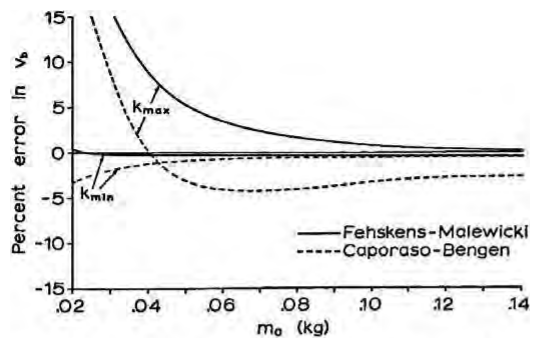
\includegraphics[width=0.8\textwidth,height=0.85\textheight,keepaspectratio]{figures/ch4/fig05a.png}
  \figurepanel{a}
  \caption{Burnout velocity error of approximate methods for vertical flight; models using Type B14
    engine.}
  \label{ch4:fig:5a}
\end{figure}

\begin{figure}[htbp]
  \centering
  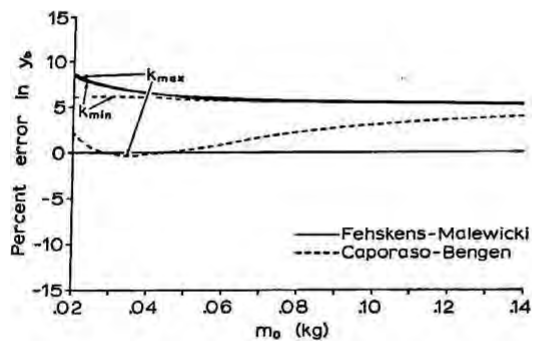
\includegraphics[width=0.8\textwidth,height=0.85\textheight,keepaspectratio]{figures/ch4/fig05b.png}
  \figurepanel{b}
  \caption{Burnout altitude error of approximate methods for vertical flight; models using Type B14
    engine.}
  \label{ch4:fig:5b}
\end{figure}

\begin{figure}[htbp]
  \centering
  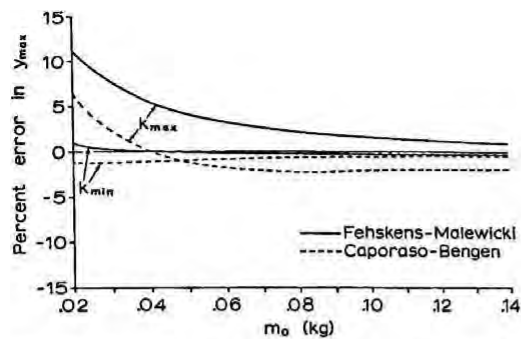
\includegraphics[width=0.8\textwidth,height=0.85\textheight,keepaspectratio]{figures/ch4/fig05c.png}
  \figurepanel{c}
  \caption{Maximum altitude error of approximate methods for vertical flight; models using Type B14
    engine.}
  \label{ch4:fig:5c}
\end{figure}

\begin{figure}[htbp]
  \centering
  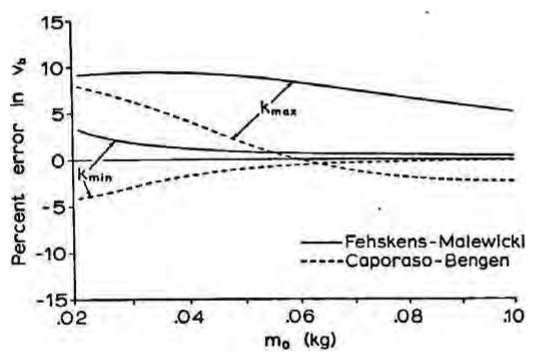
\includegraphics[width=0.8\textwidth,height=0.85\textheight,keepaspectratio]{figures/ch4/fig06a.png}
  \figurepanel{a}
  \caption{Burnout velocity error of approximate methods for vertical flight; models using Type B4 engine.}
  \label{ch4:fig:6a}
\end{figure}

\begin{figure}[htbp]
  \centering
  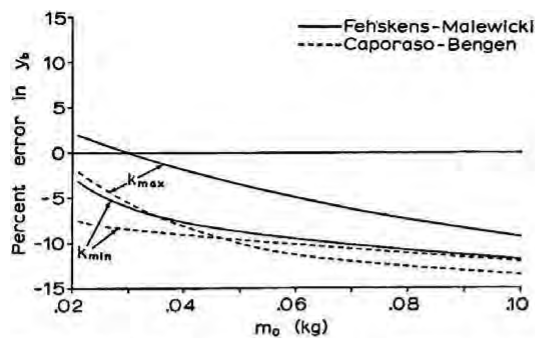
\includegraphics[width=0.8\textwidth,height=0.85\textheight,keepaspectratio]{figures/ch4/fig06b.png}
  \figurepanel{b}
  \caption{Burnout altitude error of approximate methods for vertical flight; models using Type B4 engine.}
  \label{ch4:fig:6b}
\end{figure}

\begin{figure}[htbp]
  \centering
  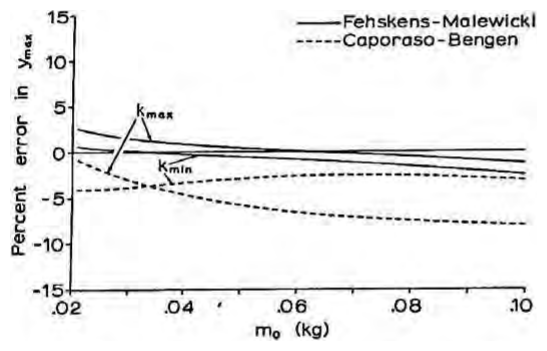
\includegraphics[width=0.8\textwidth,height=0.85\textheight,keepaspectratio]{figures/ch4/fig06c.png}
  \figurepanel{c}
  \caption{Maximum altitude error of approximate methods for vertical flight; models using Type B4 engine.}
  \label{ch4:fig:6c}
\end{figure}

\begin{figure}[htbp]
  \centering
  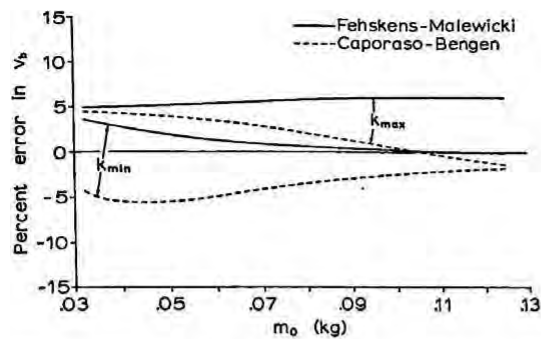
\includegraphics[width=0.8\textwidth,height=0.85\textheight,keepaspectratio]{figures/ch4/fig07a.png}
  \figurepanel{a}
  \caption{Burnout velocity error of approximate methods for vertical flight; models using Type D4 engine.}
  \label{ch4:fig:7a}
\end{figure}

\begin{figure}[htbp]
  \centering
  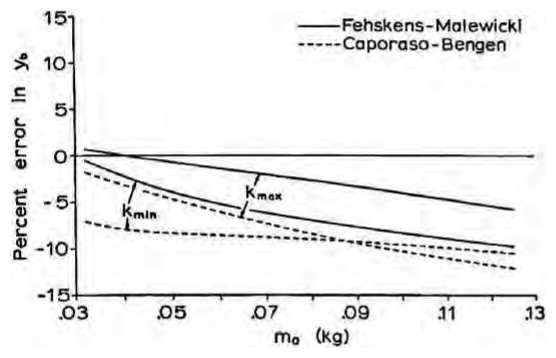
\includegraphics[width=0.8\textwidth,height=0.85\textheight,keepaspectratio]{figures/ch4/fig07b.png}
  \figurepanel{b}
  \caption{Burnout altitude error of approximate methods for vertical flight; models using Type D4 engine.}
  \label{ch4:fig:7b}
\end{figure}

\begin{figure}[htbp]
  \centering
  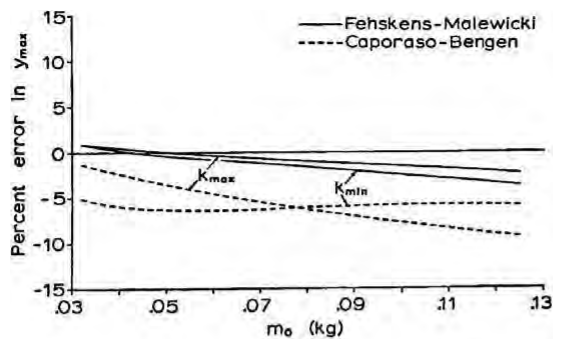
\includegraphics[width=0.8\textwidth,height=0.85\textheight,keepaspectratio]{figures/ch4/fig07c.png}
  \figurepanel{c}
  \caption{Maximum altitude error of approximate methods for vertical flight; models using Type D4 engine.}
  \label{ch4:fig:7c}
\end{figure}

\begin{figure}[htbp]
  \centering
  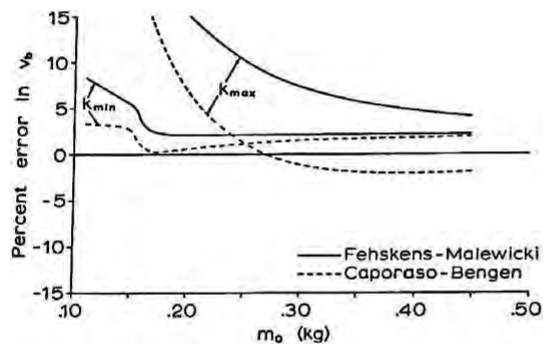
\includegraphics[width=0.8\textwidth,height=0.85\textheight,keepaspectratio]{figures/ch4/fig08a.png}
  \figurepanel{a}
  \caption{Burnout velocity error of approximate methods for vertical flight; models using Type F100
    engine. An additional error is incurred for values of $m_o$ below 0.17 kg due to transonic drag
    divergence, in the $k_{\min}$ cases.}
  \label{ch4:fig:8a}
\end{figure}

\begin{figure}[htbp]
  \centering
  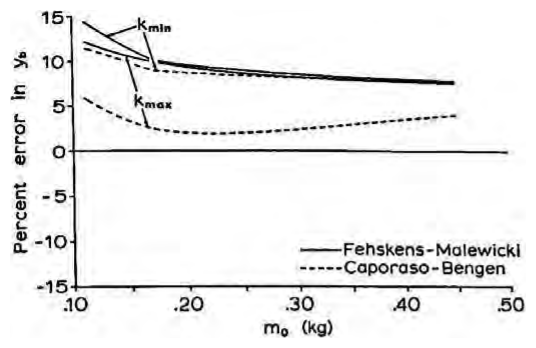
\includegraphics[width=0.8\textwidth,height=0.85\textheight,keepaspectratio]{figures/ch4/fig08b.png}
  \figurepanel{b}
  \caption{Burnout altitude error of approximate methods for vertical flight; models using Type F100
    engine. An additional error is incurred for values of $m_o$ below 0.17 kg due to transonic drag
    divergence, in the $k_{\min}$ cases.}
  \label{ch4:fig:8b}
\end{figure}

\begin{figure}[htbp]
  \centering
  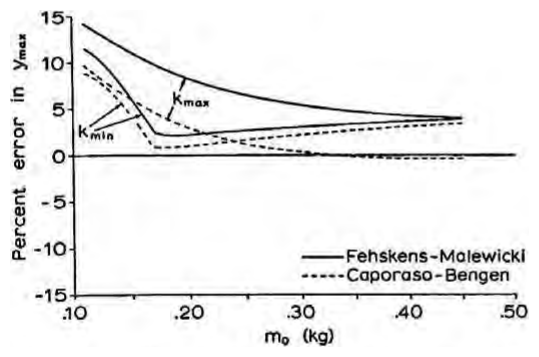
\includegraphics[width=0.8\textwidth,height=0.85\textheight,keepaspectratio]{figures/ch4/fig08c.png}
  \figurepanel{c}
  \caption{Maximum altitude error of approximate methods for vertical flight; models using Type F100
    engine. An additional error is incurred for values of $m_o$ below 0.17 kg due to transonic drag
    divergence, in the $k_{\min}$ cases.}
  \label{ch4:fig:8c}
\end{figure}

\begin{figure}[htbp]
  \centering
  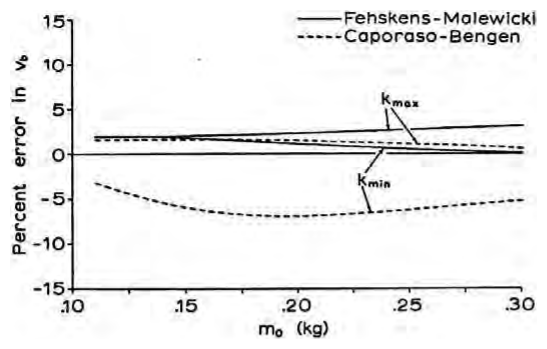
\includegraphics[width=0.8\textwidth,height=0.85\textheight,keepaspectratio]{figures/ch4/fig09a.png}
  \figurepanel{a}
  \caption{Burnout velocity error of approximate methods for vertical flight; models using Type F7 engine.}
  \label{ch4:fig:9a}
\end{figure}

\begin{figure}[htbp]
  \centering
  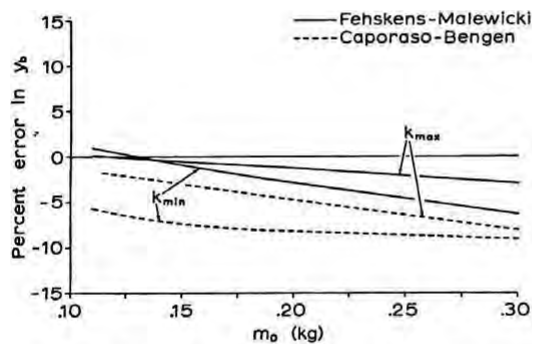
\includegraphics[width=0.8\textwidth,height=0.85\textheight,keepaspectratio]{figures/ch4/fig09b.png}
  \figurepanel{b}
  \caption{Burnout altitude error of approximate methods for vertical flight; models using Type F7 engine.}
  \label{ch4:fig:9b}
\end{figure}

\begin{figure}[htbp]
  \centering
  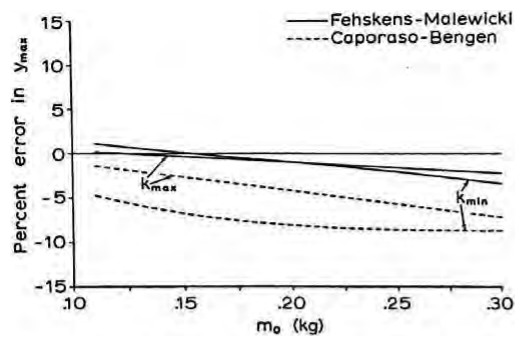
\includegraphics[width=0.8\textwidth,height=0.85\textheight,keepaspectratio]{figures/ch4/fig09c.png}
  \figurepanel{c}
  \caption{Maximum altitude error of approximate methods for vertical flight; models using Type F7 engine.}
  \label{ch4:fig:9c}
\end{figure}
